\chapter{Related Work}\label{ch:relatedWork}
Several commercial certificate authorities provide email and more generally client certificates for users.
Additionally, some corporations even offer organizational certificate management solutions.
E.g.\ Comodo\footnote{\url{https://www.comodo.com/home/email-security/free-email-certificate.php}},
Digicert\footnote{\url{https://www.digicert.com/client-certificates/}}, and
Globalsign\footnote{\url{https://www.globalsign.com/de-de/sichere-email/}} all offer solutions, that integrate with
commonly used user management solutions for organizations (Active Directory).
All commercially available solutions are unfortunately closed-source, which is usually a red flag for encryption related
and trust providing applications, since it hinders independent audition and source code review for potential security
holes.
Additionally, the service is comparatively expensive with around 10€ per user and year, which is rather unappealing for
organizations the size of TUM with almost 50k users.

A more recent open source project, providing encryption certification services is Let's Encrypt.
The Let's Encrypt system provides a way to automatically provide x509 certificates for client to server communication,
e.g.\ for HTTPS\@.
This system works via an Automatic Certificate Management Environment (ACME), which is specified in an IETF standard
working draft~\cite{letsencrypteacme}.

\begin{figure}[hb]
    \centering
    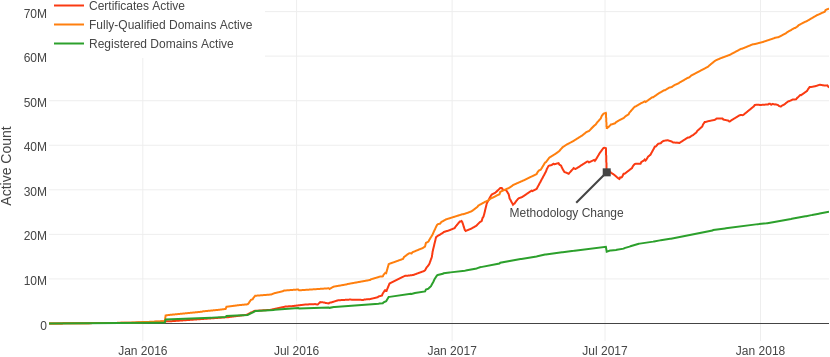
\includegraphics[width=.905\textwidth]{figures/letsencryptusers.png}
    \caption{Let's Encrypt users until mid 2018~\cite{letsencryptstats}}
    \label{fig:letsencrypt}
\end{figure}

This project is already immensely successful, providing over 50 Million active certificates, as of March 2018 (see
\Cref{fig:letsencrypt})
However, this system is not intended for the general population, since the validation challenges are not end-user
focused, but mostly for web servers.
X.509 certificates, as issued by Let's Encrypt can generally be used for email security with S/MIME\@.
Since this is not the focus of Let's Encrypt, they also do not issue certificates, that would be usable for email
encryption.

More work about how email encryption certificates can be managed in a organization has been done by the TUM Secure
Email and User Certification Project, with the works
of~\citet{hauner2016interoperability, jagdish2016certservice, straub2016directoryservice, maier2015multidevice}.
Maximilian Meier explored secure email communication with multiple devices, where he analyzed the requirements of
users and surveyed different implementations, that try to satisfy those requirements.
Straub and Jagdish worked on a combined system, which allows storage and management of digital certificates using a Java
backend with a web frontend.
In their work, they created a basic system, which can be used to store and manage certificates, but does not integrate
well with existing infrastructure in organizations.
In the most recent work, Valentin Hauner worked on extending this system to publish certificates via different exchange
protocols.
